%%% Моделирование %%%
\section{Моделирование}

Во время селективного спекания порошкового металла под воздействием лазеров или пучков электронов, энергия от них вызывает нагрев частиц порошка на поверхности. 
При этом в точке воздействия источника энергии образуется область, где образуется бассейн рассплавленного металла, который в последествии застывает и соединяется с предыдущими областями, создавая непрерывную деталь.

Моделирование поведения компоненнтов в этой области -- потери от испарения, диффузия, конвекция, плавление и застывание -- позволяет судить об итоговом составе получившейся детали и, как следствие, о её механических свойствах и микроструктуре.

\subsection{Нульмерная модель}

В процессе движения по засыпанному слою порошка, область расплава следует за источником и через какое-то время её размеры перестают расти и до смены направления движения сохраняются около определённого значения. 
Поэтому в данной модели рассматривается поведение концентраций компонентов в предположении бесконечно быстрой диффузии в бассейне расплава неизменной 
прямоугольной формы. На рисунке \ref{fig:zero-model} изоражена геометрическая интерпретация модели.

Уравнение на потоки \ref{eq:zero-general} и формулы для каждого потока выглядят следующим образом \ref{eq:zero-melt} - \ref{eq:lambda}:
\begin{equation}
    \label{eq:zero-general}
    \dot{m} = j_{melt} - j_{solid} - j_{evap}
\end{equation}
\begin{equation}
    \label{eq:zero-melt}
    j_{melt} = \lambda m
\end{equation}
\begin{equation}
    \label{eq:zer-sol}
    j_{solid} = \lambda m_0
\end{equation}
\begin{equation}
    \label{eq:lambda}
    \lambda = \frac{v_{beam}}{L}
\end{equation}

\noindent
здесь $v_{beam}$ -- скорость сканирования, а $m$ и $m_0$ -- текущая и начальная масса содержимого бассейна.

Таким образом уравнения \ref{eq:zero-general} - \ref{eq:lambda} в связке с уравнениями для рассчёта испарения \ref{eq:evap} - \ref{eq:cc} формируют систему, описывающую данную нульмерную модель.

Стоит отметить, что данная модель не учитвает многокомпонентности, а уравнение \ref{eq:zero-general} может быть решено аналитически:

\begin{equation}
    m = m_0 -\frac{j^{evap}}{\lambda} (1 - e^{-\lambda t})
\end{equation}
\begin{equation}
    \lim_{t\rightarrow \infty } m = m_0 - \frac{j^{evap}}{\lambda}
\end{equation}

\addimg{zero-model-view.pdf}{0.8}{Нульмерная модель бассейна расплава. Здесь $j_{evap}$ -- поток испарения, $j_{melt}, j_{solid}$ -- потоки приходящего (плавящегося) и уходящего (застывающего) вещества соотвественно, определяемые скоростью движения источника.}{fig:zero-model}

На рис. \ref{fig:anal-solution} изображено решение для бассейна расплавленного алюминия температурой 3000К, диаметром источника 0.1 мм, размеры бассейна раплава -- 1000\times300\times100 мкм -- длина, ширина и глубина соответственно. Параметры матриала, необходимые для рассчёта испарения были взяты из работы \cite{klassen2018simulation}.

\addimg{anal_solution.pdf}{1.0}{Аналитическое решение уравнения \ref{eq:zero-general}}{fig:anal-solution}

Уравнение для 2 компонент:

\begin{equation}
    \label{eq:zero-double-comp}
    \dot{m_{\alpha}} = -j_{\alpha} \gamma^{\text{акт}}_{\alpha} \frac{\mu_{\alpha}}{m_{\alpha}}\frac{1}{\sum\limits_{\alpha} \frac{\mu_{\alpha}}{m_{\alpha}}} + \lambda (m_{\alpha}^0 - m_{\alpha})
\end{equation}

\addimg{thesis-w-3000.pdf}{1.0}{Численное решение уравнения \ref{eq:zero-general}}{fig:test}

\begin{figure}
    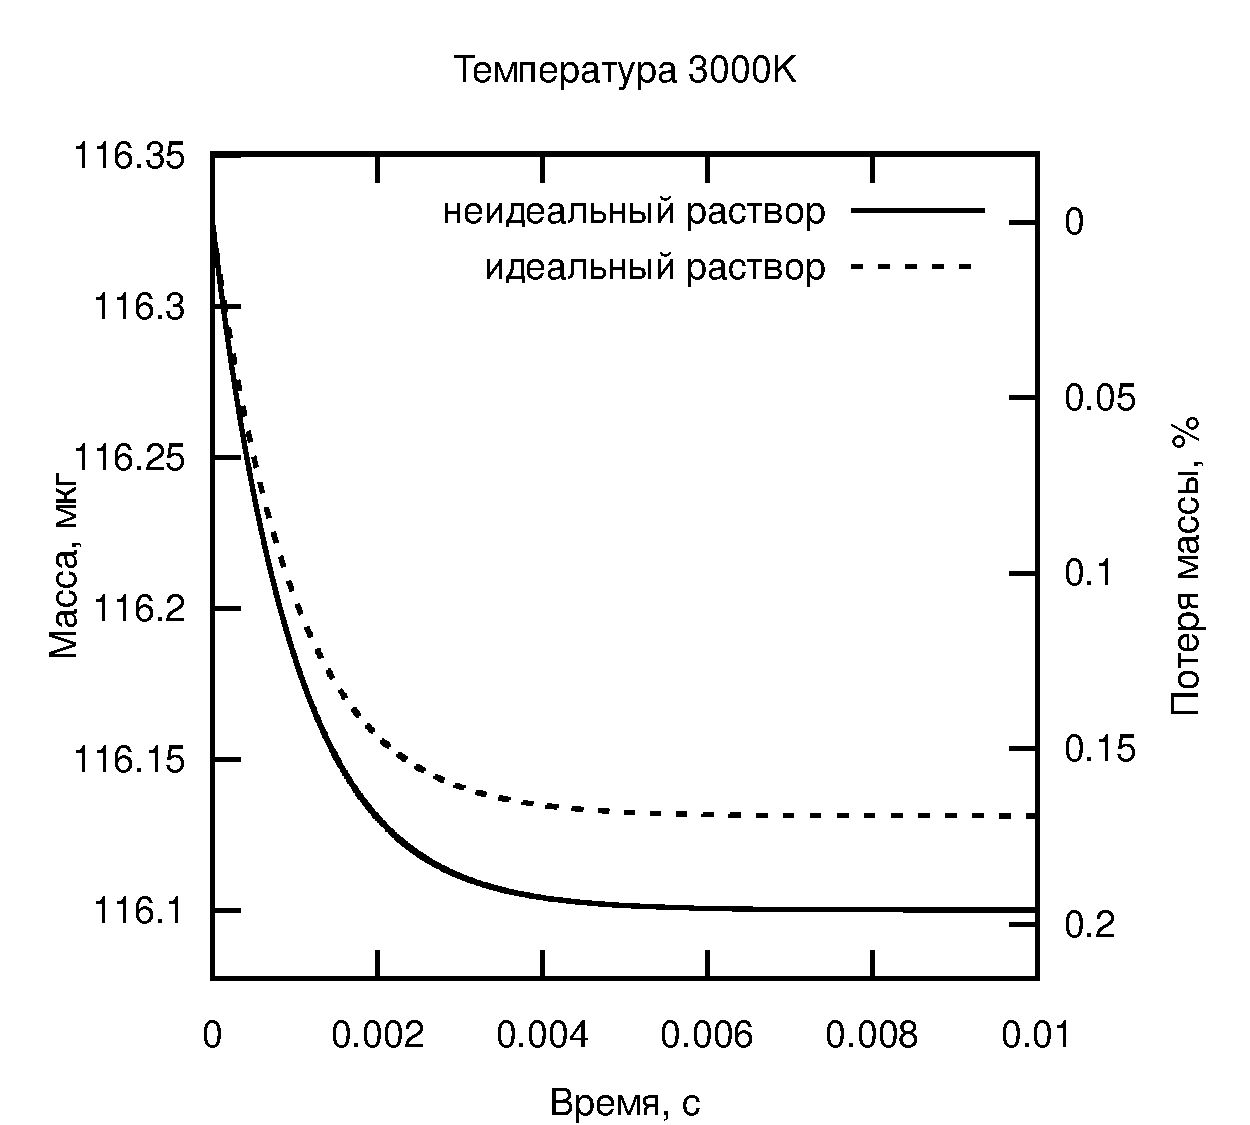
\includegraphics[width=.5\textwidth]{thesis-w-3000.pdf}\hfill
    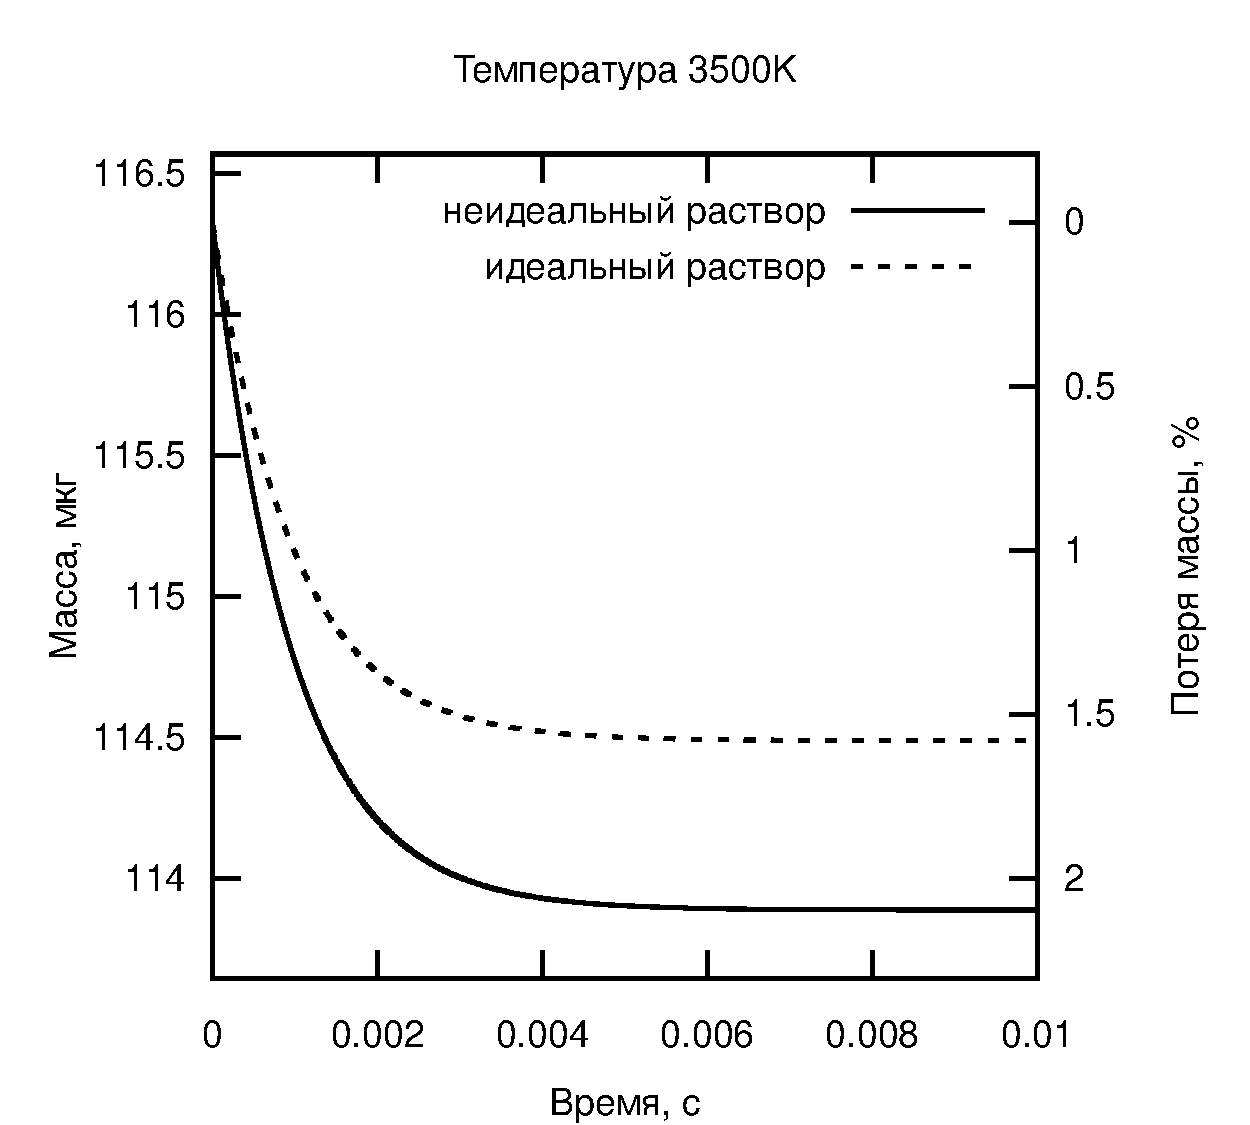
\includegraphics[width=.5\textwidth]{thesis-w-3500.pdf}\hfill
    \\[\smallskipamount]
    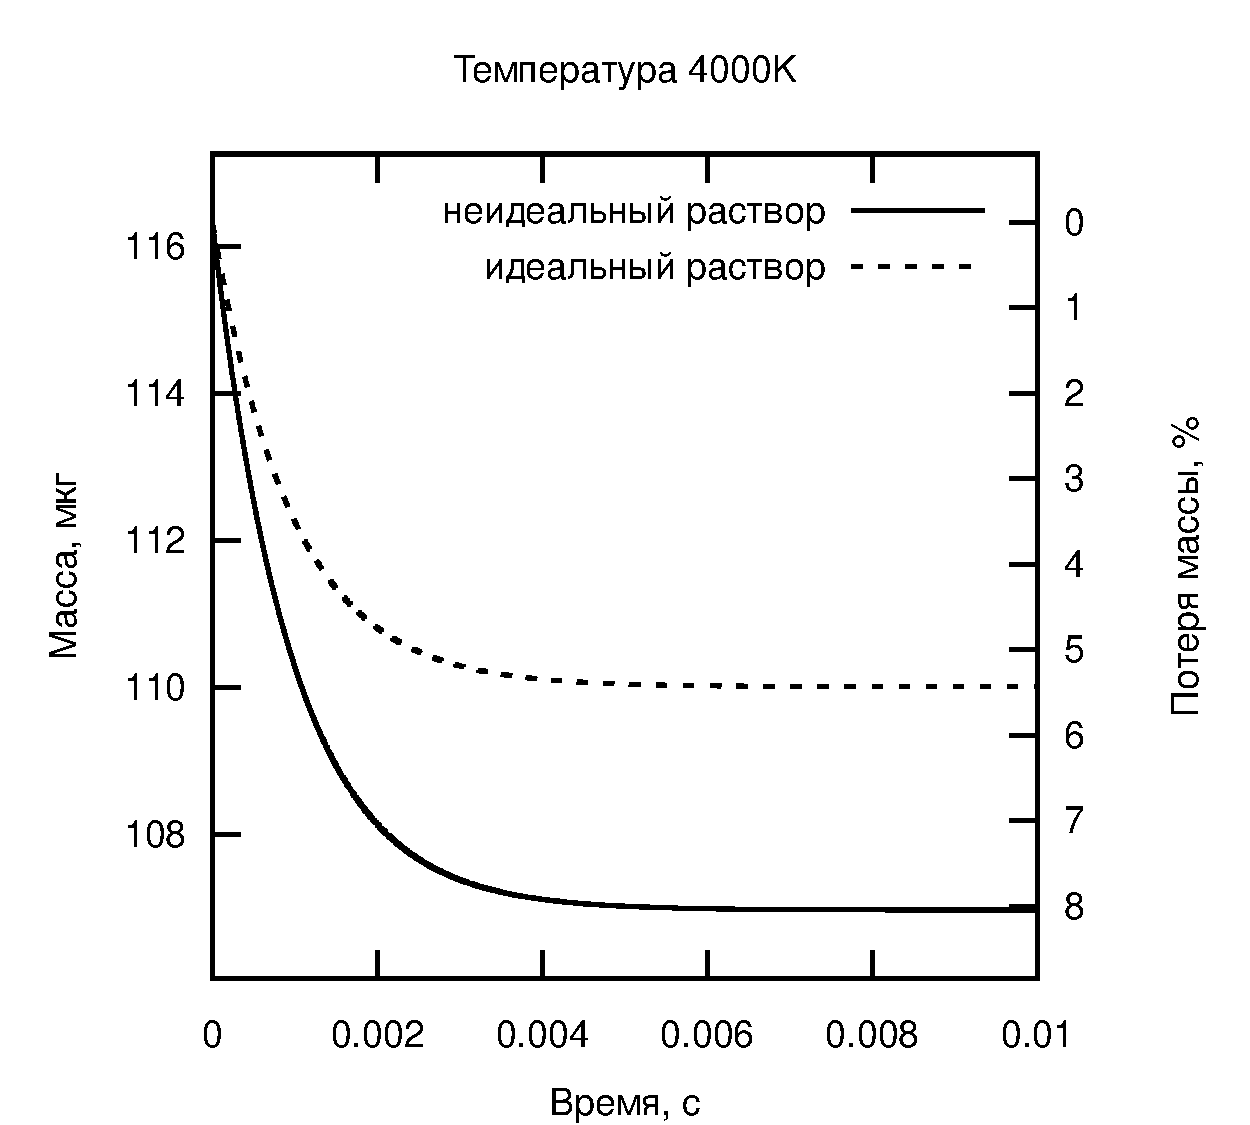
\includegraphics[width=.5\textwidth]{thesis-w-4000.pdf}\hfill
    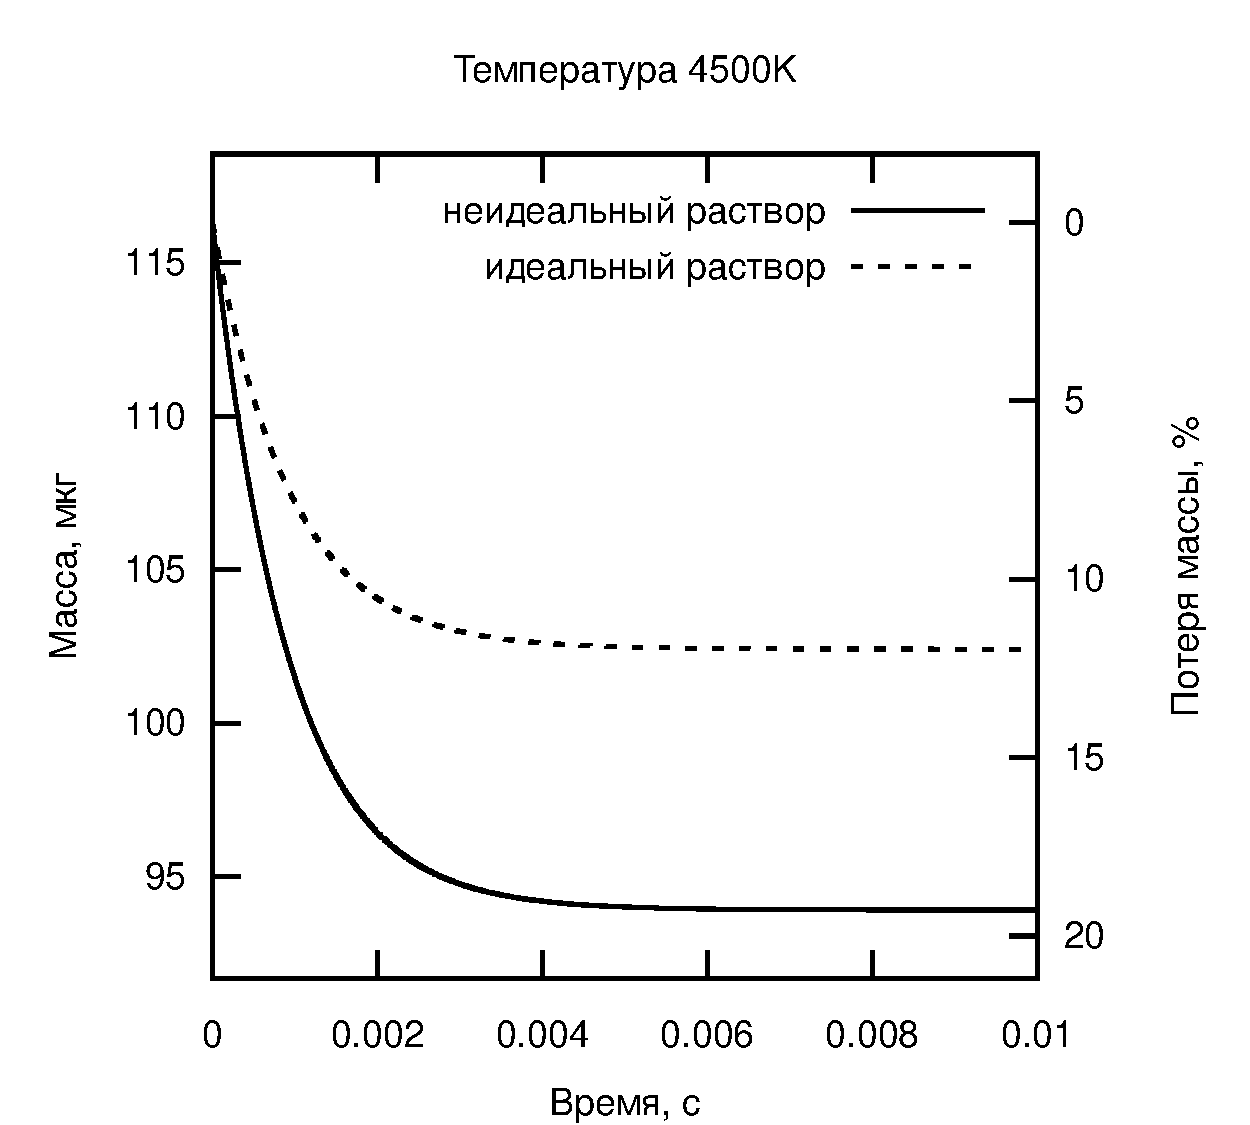
\includegraphics[width=.5\textwidth]{thesis-w-4500.pdf}\hfill
\end{figure}


\begin{figure}
    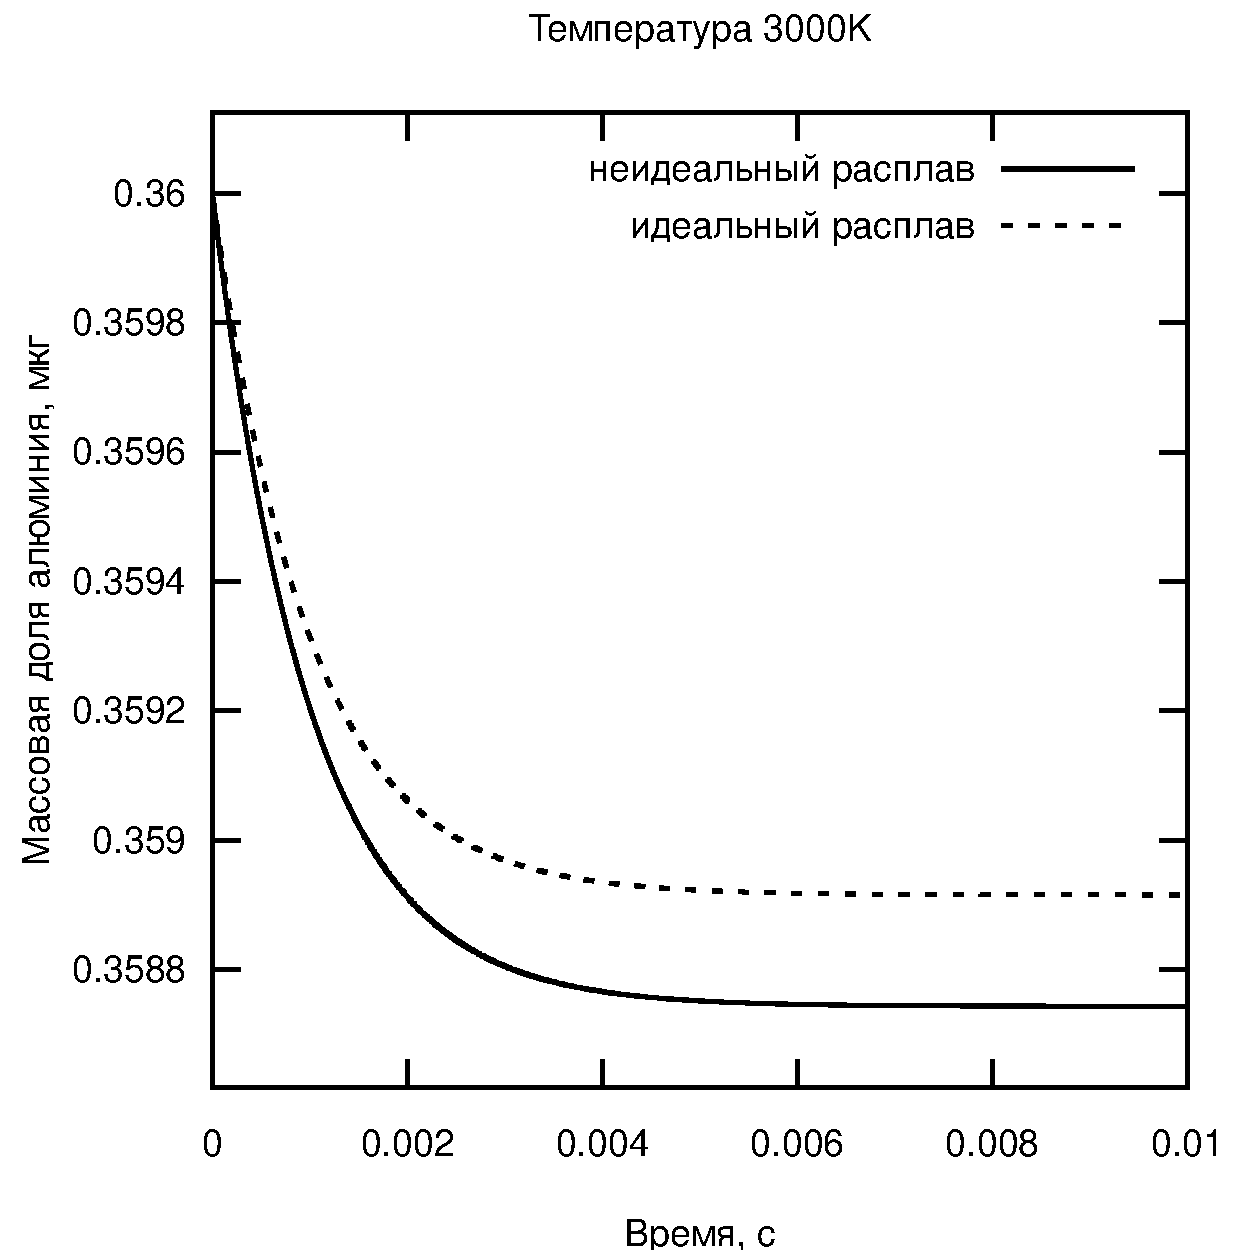
\includegraphics[width=.5\textwidth]{thesis-cwwo-3000.pdf}\hfill
    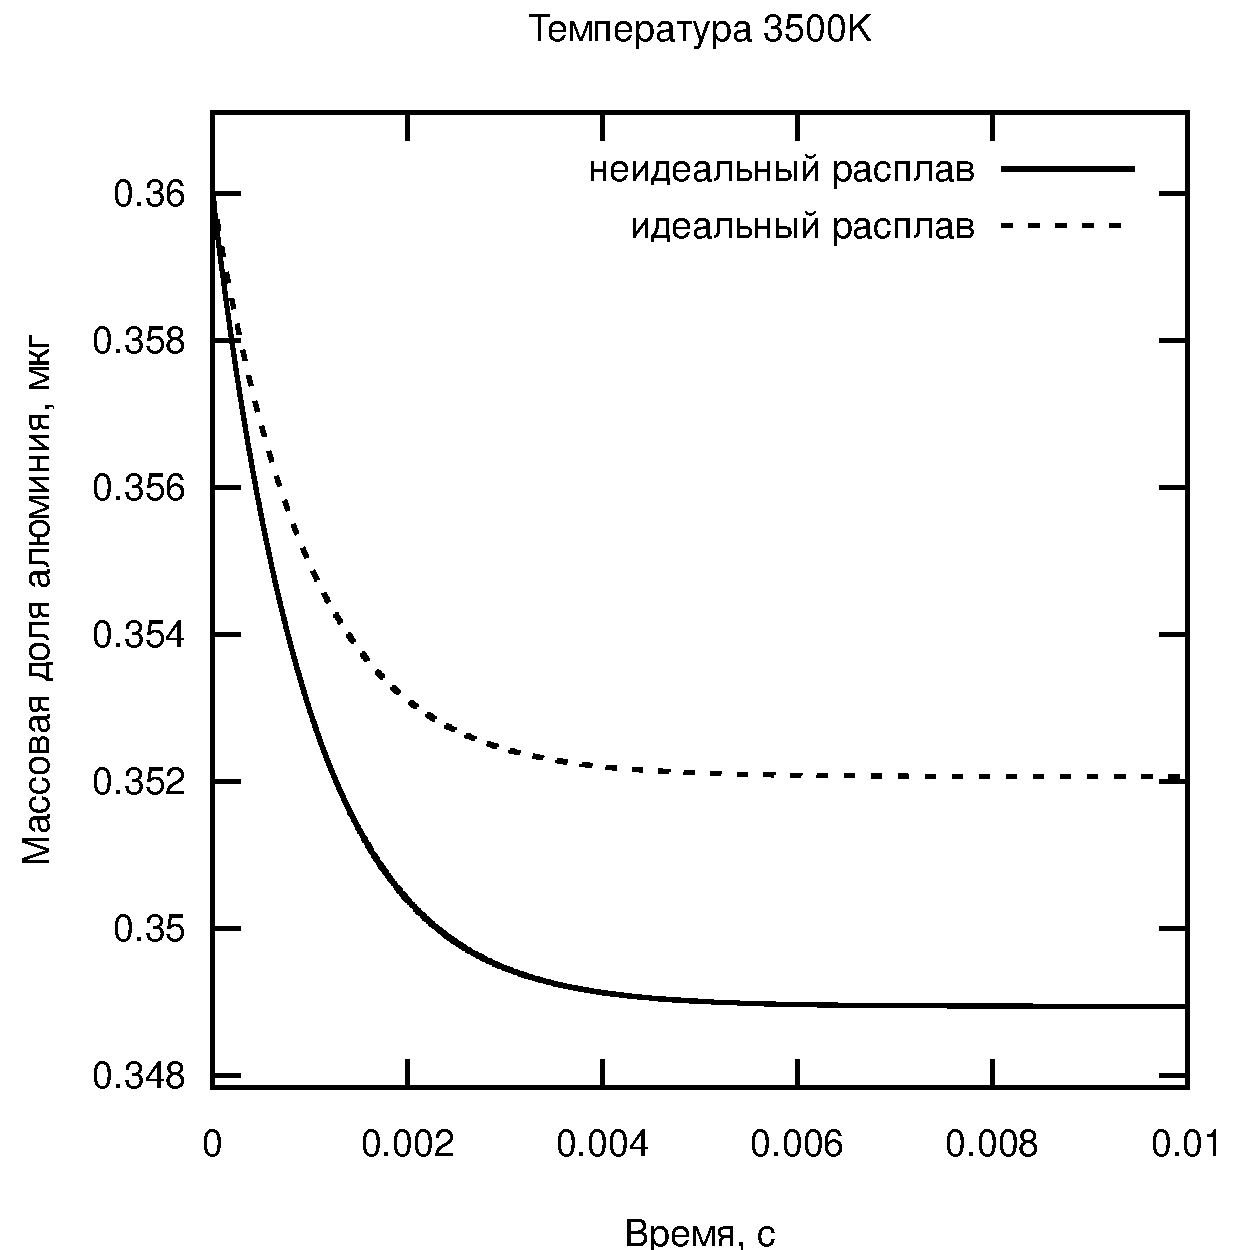
\includegraphics[width=.5\textwidth]{thesis-cwwo-3500.pdf}\hfill
    \\[\smallskipamount]
    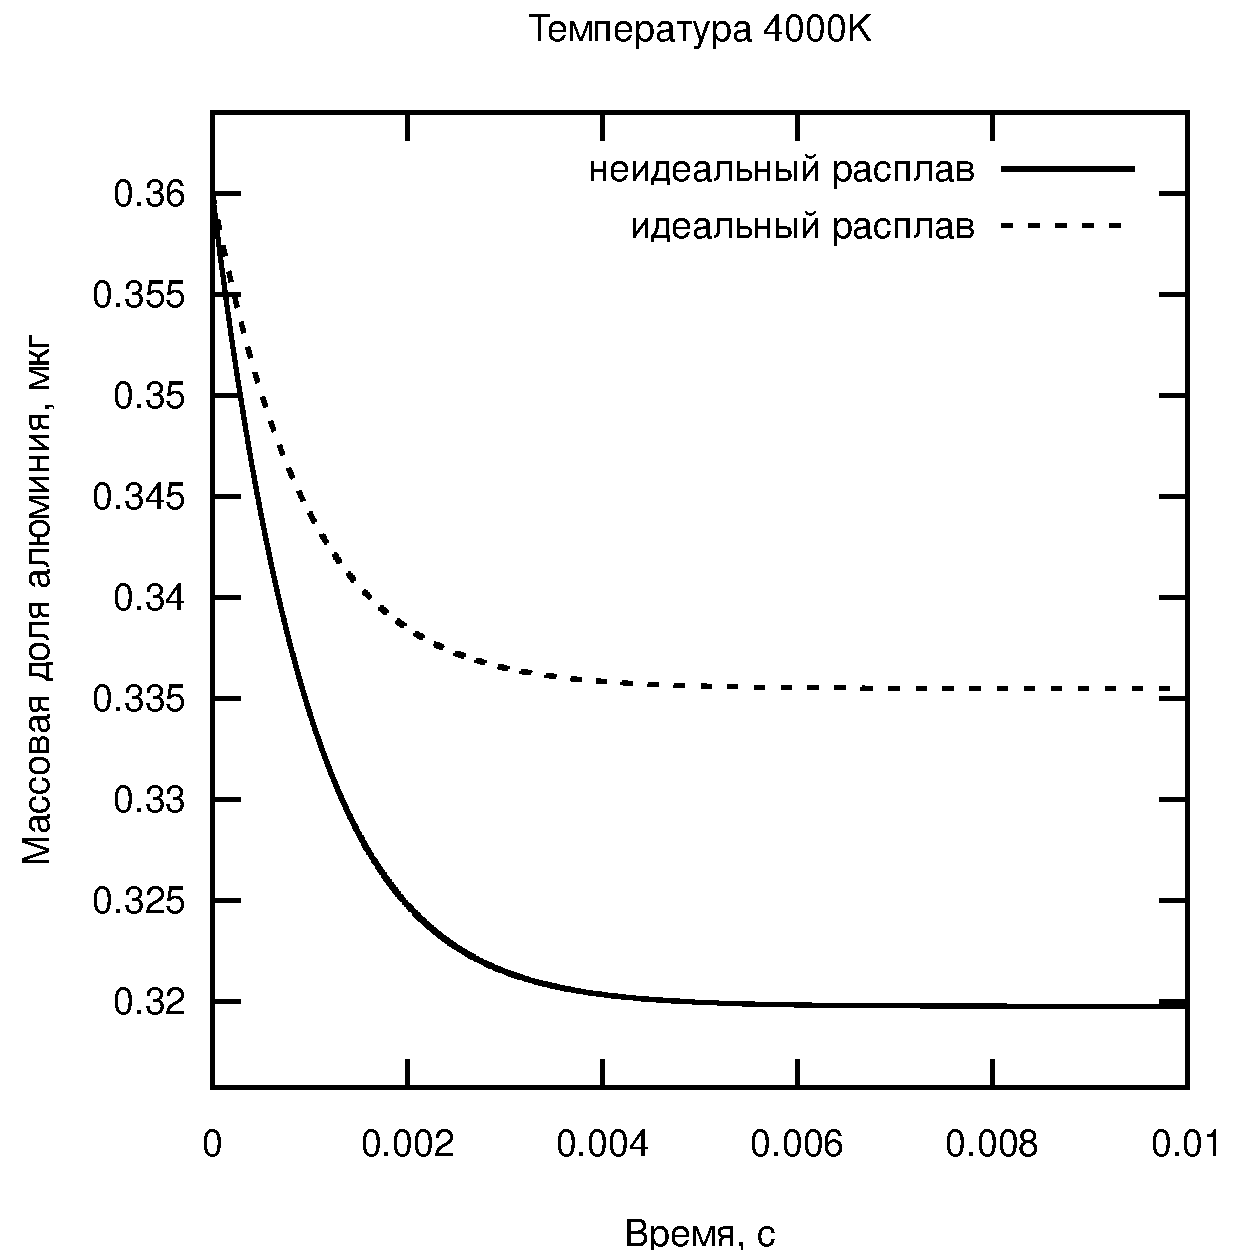
\includegraphics[width=.5\textwidth]{thesis-cwwo-4000.pdf}\hfill
    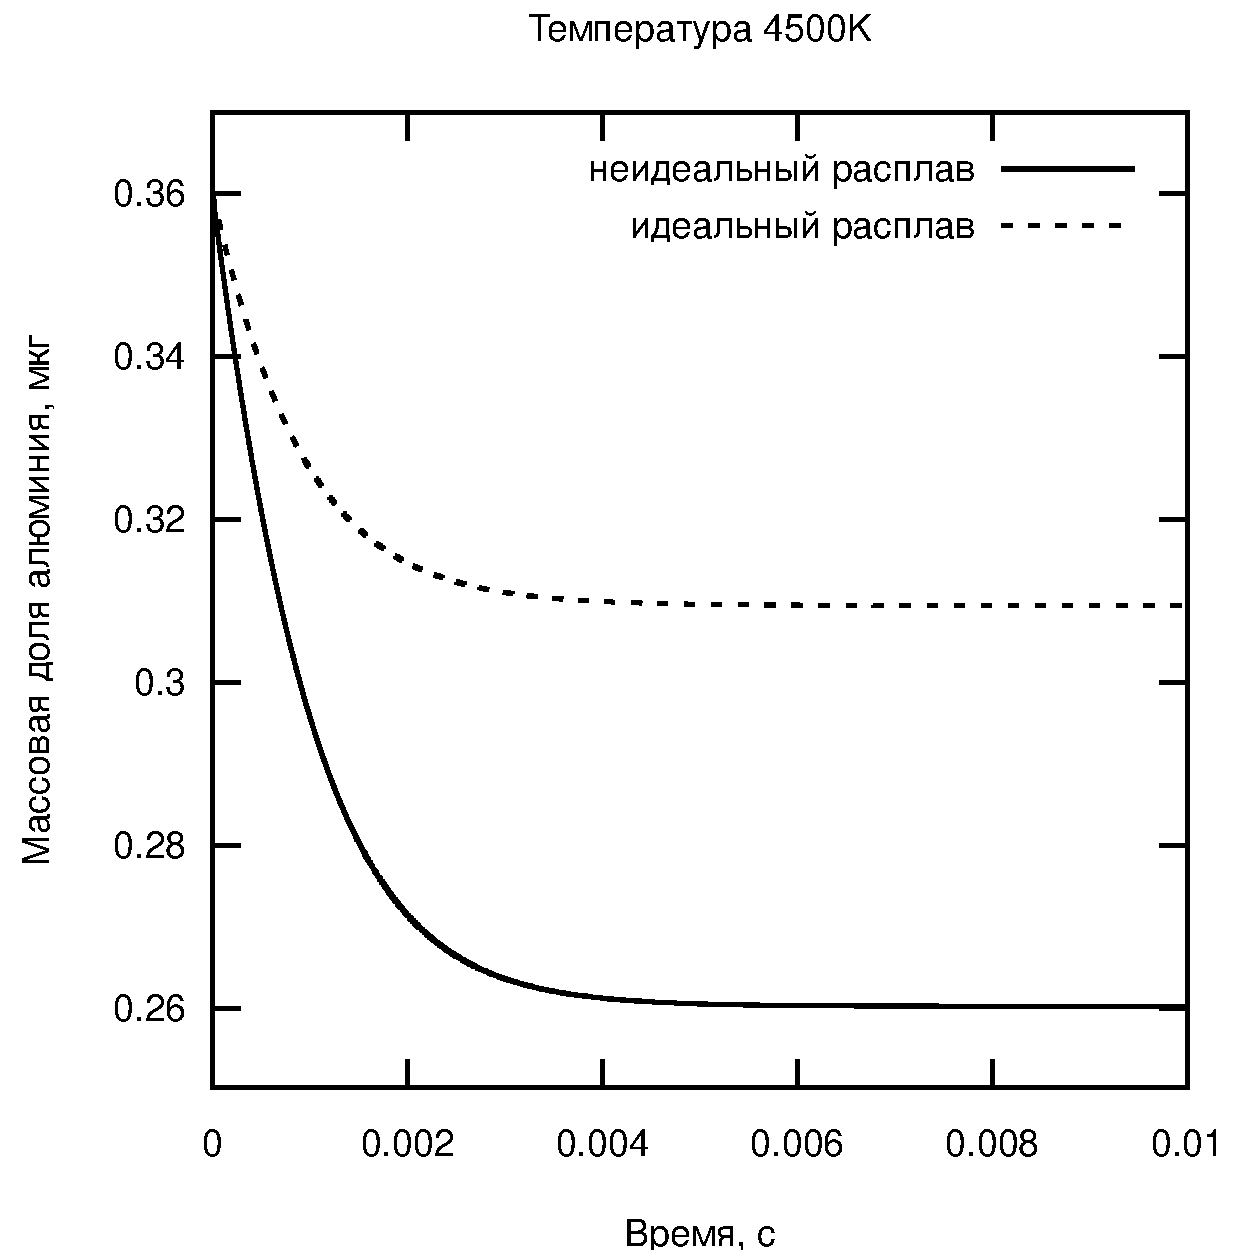
\includegraphics[width=.5\textwidth]{thesis-cwwo-4500.pdf}\hfill
\end{figure}
\begin{figure}
    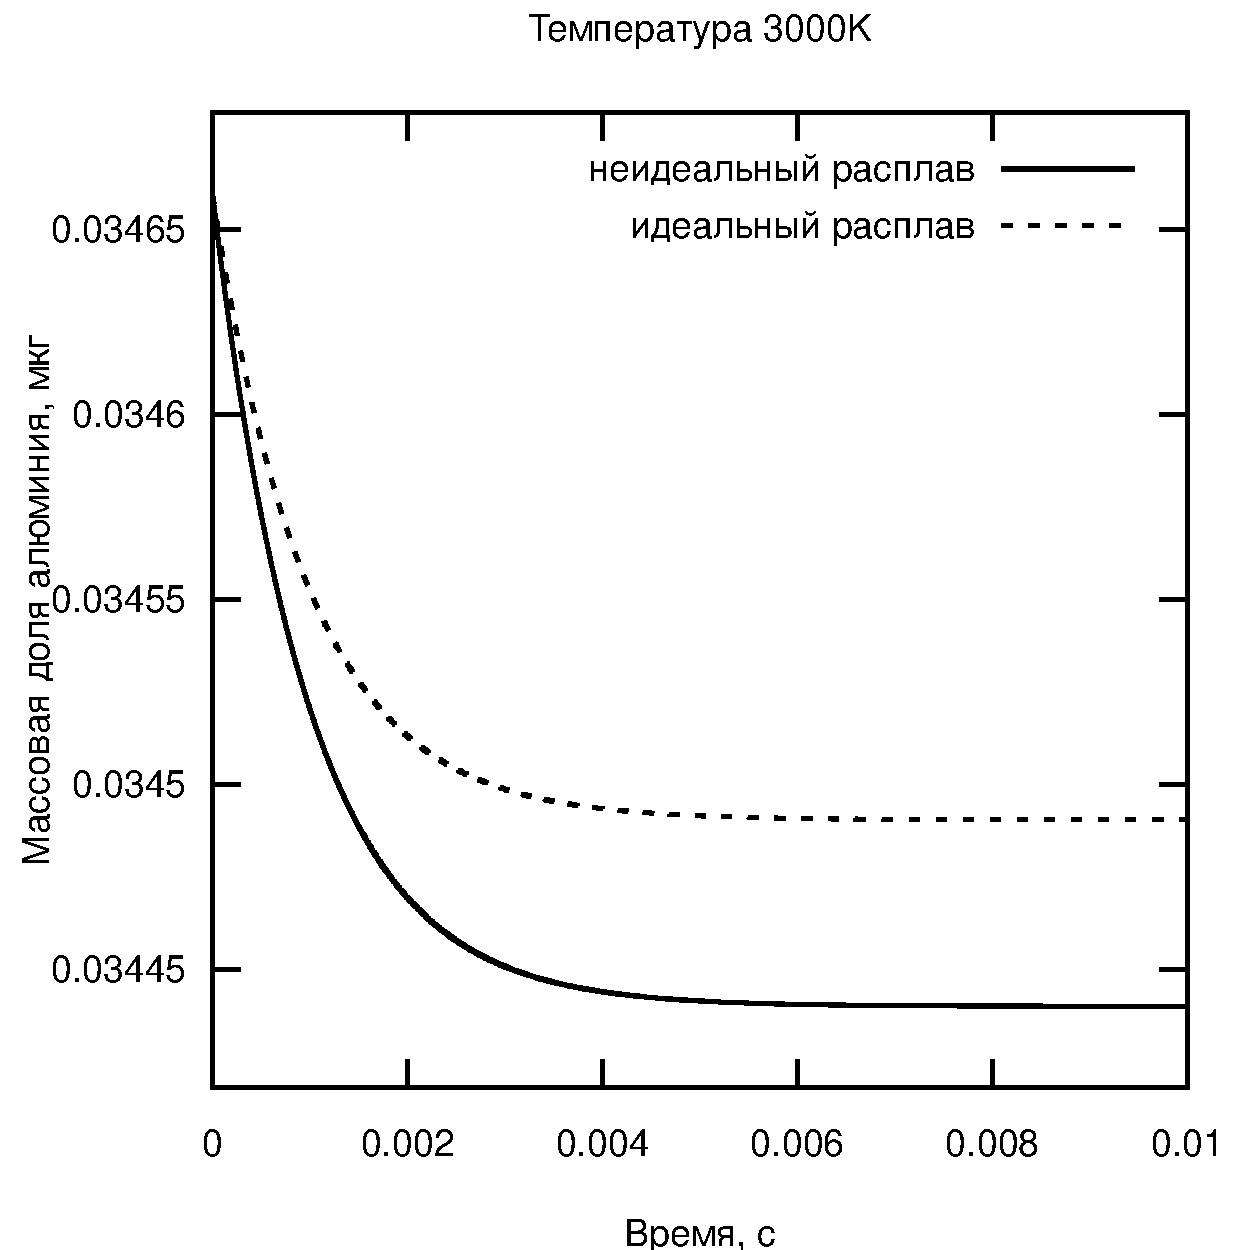
\includegraphics[width=.5\textwidth]{thesis-cwwo6-3000.pdf}\hfill
    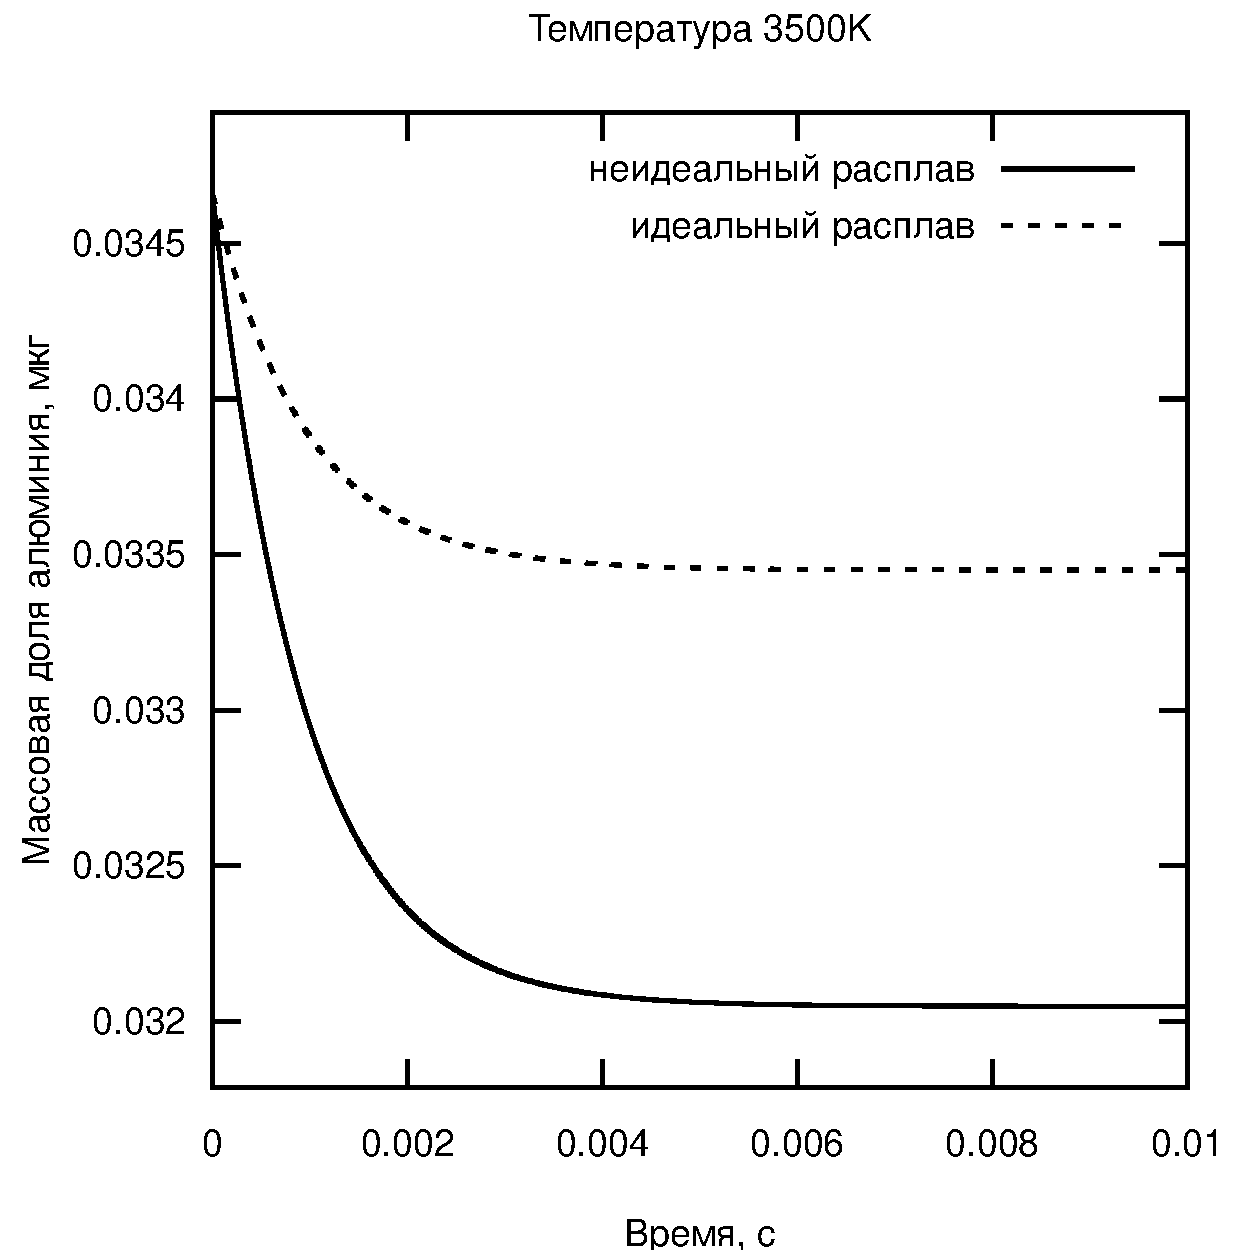
\includegraphics[width=.5\textwidth]{thesis-cwwo6-3500.pdf}\hfill
    \\[\smallskipamount]
    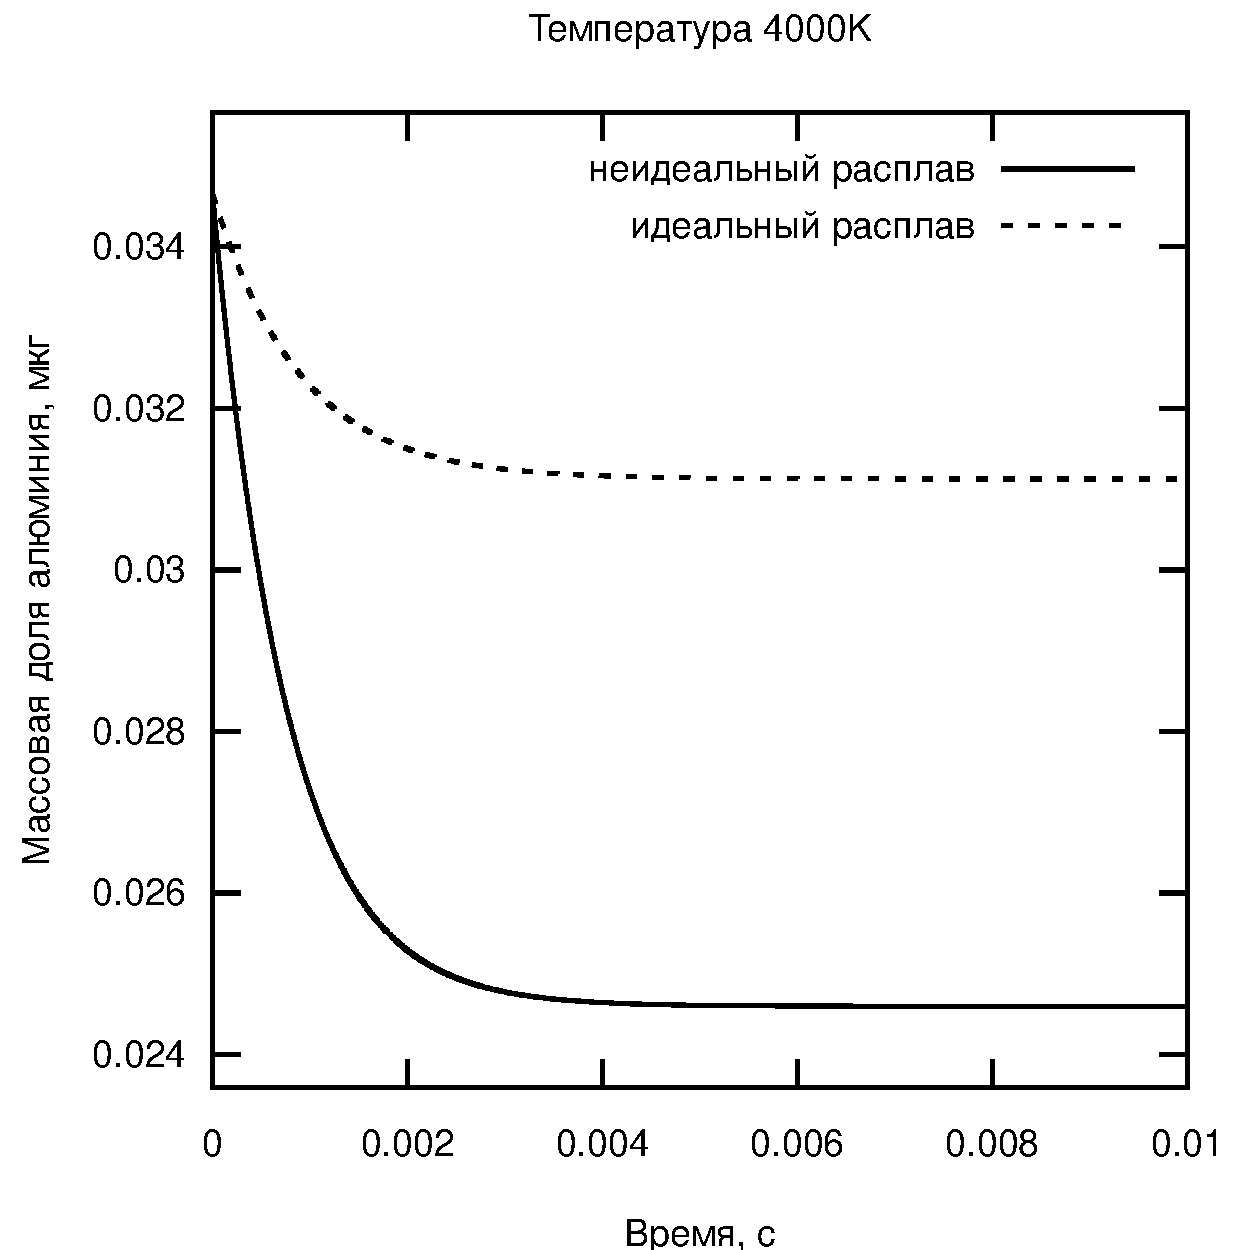
\includegraphics[width=.5\textwidth]{thesis-cwwo6-4000.pdf}\hfill
    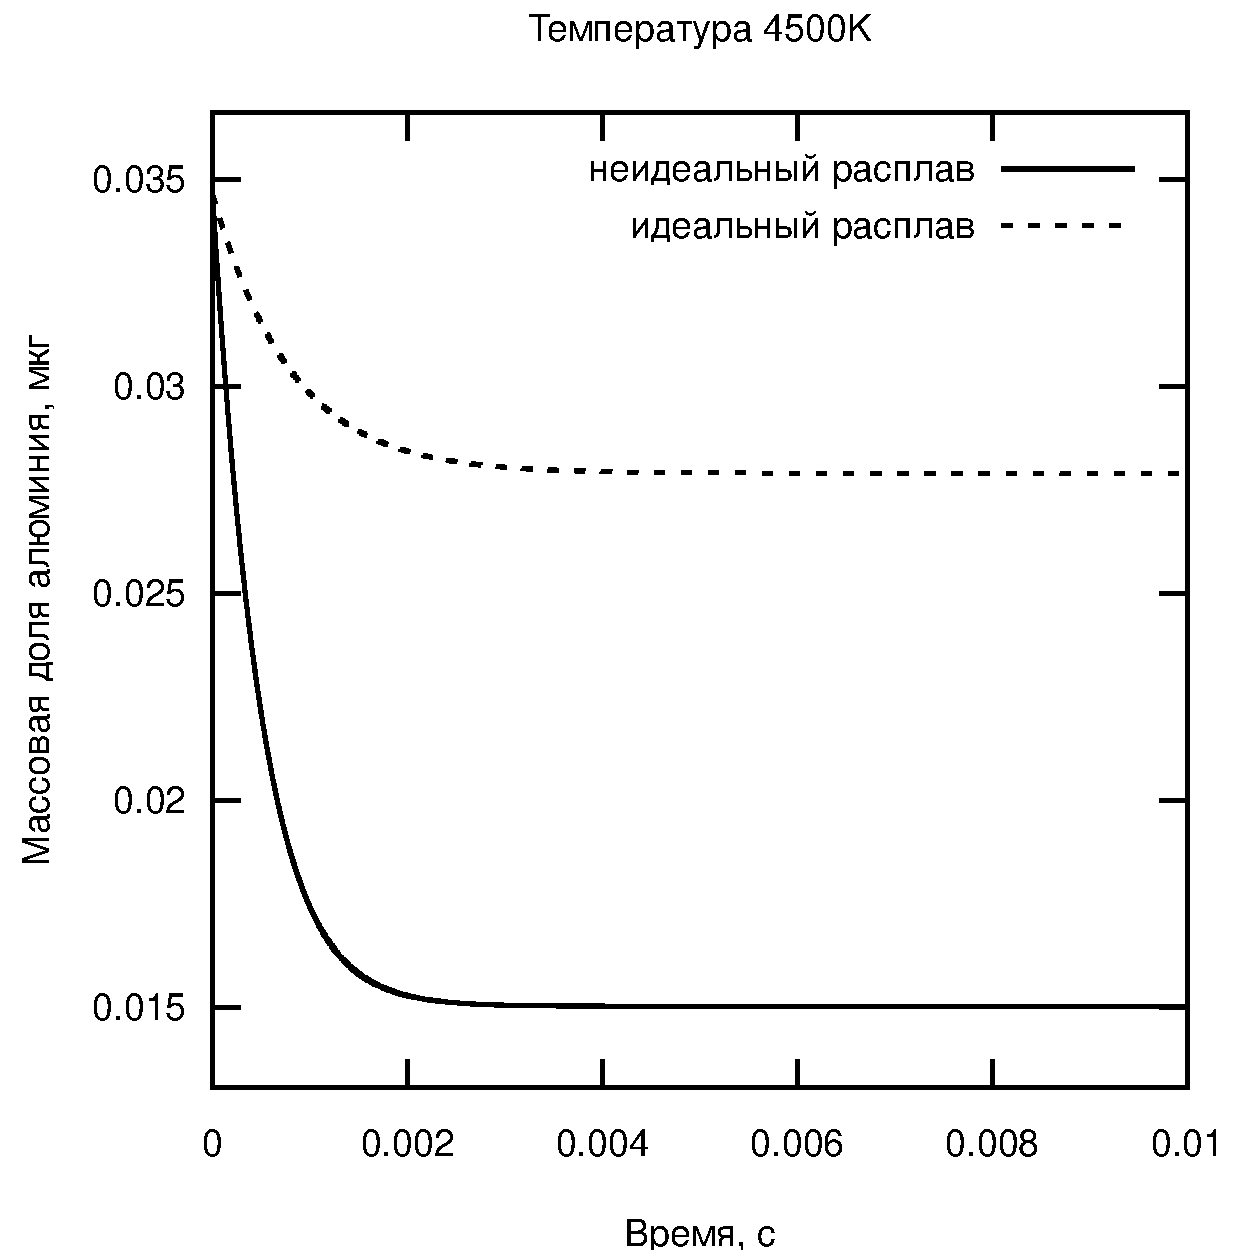
\includegraphics[width=.5\textwidth]{thesis-cwwo6-4500.pdf}\hfill
\end{figure}



\clearpage